\documentclass[11pt,a4paper]{article}
\usepackage[margin=1in]{geometry}
\usepackage[T1]{fontenc}
\usepackage[utf8]{inputenc}
\usepackage{lmodern}
\usepackage{microtype}
\usepackage{amsthm,amsmath,amssymb,amsfonts}
\usepackage{mathtools}
\usepackage{booktabs}
\usepackage{tikz}
\usetikzlibrary{arrows.meta,decorations.pathreplacing}
\usepackage[colorlinks,urlcolor=blue!50!black,linkcolor=blue!50!black,citecolor=green!40!black]{hyperref}
\usepackage{cleveref}

\newtheorem{theorem}{Theorem}
\newtheorem{lemma}{Lemma}
\newtheorem{observation}{Observation}
\newtheorem{corollary}{Corollary}
\theoremstyle{definition}
\newtheorem{definition}{Definition}
\newtheorem{construction}{Construction}
\theoremstyle{plain}
\newtheorem*{characterization}{Characterization}
\newtheorem*{karp}{Theorem (Karp)}
\crefname{observation}{Observation}{Observations}
\Crefname{observation}{Observation}{Observations}
\crefname{construction}{Construction}{Constructions}
\Crefname{construction}{Construction}{Constructions}

\newcommand{\doi}[1]{DOI: \href{https://doi.org/#1}{\nolinkurl{#1}}}
\newcommand{\FF}{FF(1,m)\mid\mid\textstyle\sum_j w_jZ_j}
\newcommand{\FFu}{FF(1,m)\mid\mid\textstyle\sum_j Z_j}
\newcommand{\qmax}{q_{\max}}
\newcommand{\wmax}{w_{\max}}
\newcommand{\HS}{\textsc{Hitting Set}}
\newcommand{\SAT}{\textsc{Sat}}
\newcommand{\NP}{\textnormal{\textsf{NP}}}
\newcommand{\Wtwo}{\textnormal{\textsf{W[2]}}}
\newcommand{\FPT}{\textnormal{\textsf{FPT}}}
\newcommand{\calJ}{\mathcal{J}}
\newcommand{\calZ}{\mathcal{Z}}
\newcommand{\vecx}{\vec{x}}

\title{Just-in-Time Scheduling in Two-Stage Flexible Flow Shops}
\author{Yuval Itzhaki \and Claude}
\date{}

\begin{document}
\maketitle

\begin{abstract}
In the two-stage flexible flow shop $\FF$ every job is first preprocessed on a single machine
and then processed on one of $m$ identical machines, and the objective is the total weight of
the jobs whose second operation ends exactly at their due date. Heeger, Hermelin, Itzhaki,
Schieber and Shabtay~\cite{HHISS26} characterize the sets of jobs that can all be completed
just in time, give five algorithms built on the characterization, and show that the problem
is strongly \NP-hard, and \Wtwo-hard for the number of machines, already for unit weights.
All of these results are proved in Lean, including the running times of the algorithms as word
RAM programs and the \NP-hardness of \HS. This note presents the scheduling results in the
notation of~\cite{HHISS26}, with links to Lean. The accompanying archive's concept pages
also document the W-hierarchy development.
\end{abstract}

\section{Introduction}

In a two-stage flexible flow shop every job is first preprocessed, without preemption, on a
single first-stage machine and then processed on one of $m$ identical second-stage machines.
Job $j$ has a preprocessing time $p_j$, a processing time $q_j$, a due date $d_j$ and a weight
$w_j$. It is \emph{just in time} if its second operation ends exactly at $d_j$, and the goal is
a schedule maximizing the total weight of the just-in-time jobs. In the three-field notation of
Graham et al.\ the problem is $\FF$. The paper~\cite{HHISS26} characterizes the sets of jobs
that can be completed just in time (\Cref{sec:model}), and builds on this characterization:

\begin{itemize}
\item a dynamic program in $O(W\cdot n^m)$ time, where $W=\sum_jw_j$ (\Cref{thm:mainDP}), and
  in $O(P\cdot n^m)$ time, where $P=\sum_jp_j$ (\Cref{cor:P});
\item two further programs in $O(W\cdot2^{\omega}\cdot n)$ and $O(W\cdot m^{\qmax}\cdot n)$ time,
  where $\omega$ is the largest number of jobs whose second operations overlap at one instant
  and $\qmax=\max_jq_j$ (\Cref{thm:secondaryDPs});
\item for equal preprocessing times, a program in $O(n^{m+1})$ time (\Cref{cor:uniform}), a
  greedy in $O(n\log n)$ time for unit weights, and an integer program with a totally
  unimodular matrix for the weighted case on proper instances (\Cref{thm:Uniform});
\item a fully polynomial-time approximation scheme when $m$, $\omega$ or $\qmax$ is bounded
  (\Cref{thm:fptas});
\item strong \NP-hardness, and \Wtwo-hardness for $m$, already for unit weights, by a reduction
  from \HS\ (\Cref{thm:NP-hard}, \Cref{cor:W2}).
\end{itemize}

% lax begin lax-808846
Running times are statements about word RAM programs: a program is a fixed list of instructions
operating on words of $w$ bits, and its running time is the number of instructions it executes.
Each algorithm of the paper is written as such a program in the IMP+ language of the archive,
compiled by its verified compiler, and shown to compute the stated function within the stated
number of instructions. The due dates and weights are entries of the input word, so a bound
cannot be stated against the number of jobs alone: the entries must fit in words of length
$w$, and this is part of every statement below.
% lax end

\section{The Problem}\label{sec:model}

% lax begin Lax496464.FlowShop
\begin{definition}[$\FF$]
An instance consists of $n$ jobs $\calJ=\{1,\ldots,n\}$ and $m$ identical second-stage
machines. Job $j$ has a preprocessing time $p_j\in\mathbb N$ on the single first-stage machine, a
processing time $q_j\in\mathbb N$ on a second-stage machine, a due date $d_j\in\mathbb N$ and a
weight $w_j\in\mathbb N$. The two operations of a job are run in this order and without
preemption. Job $j$ is \emph{completed just in time} if its second operation ends exactly at
$d_j$, and the objective is to maximize the total weight of the jobs completed just in time.
\end{definition}
Completing job $j$ just in time pins its second operation to the interval $[s_j,d_j)$, where
$s_j=d_j-q_j$ is its \emph{start time}; the first operation must be finished by $s_j$. Two
jobs are \emph{in conflict} if their intervals overlap, and conflicting jobs cannot share a
second-stage machine. Only the jobs completed just in time matter, so a solution is the set
$\calZ$ of these jobs, and $\calZ$ is \emph{feasible} if there is a schedule completing
every job of $\calZ$ just in time. See \Cref{fig:model}.
% lax end

\begin{figure}[tb]
    \centering
    % The two-stage flexible flow shop and the two operations of a job, as two pictures set side by side
% and centered on each other. Adapted from the slide "Problem Definition".
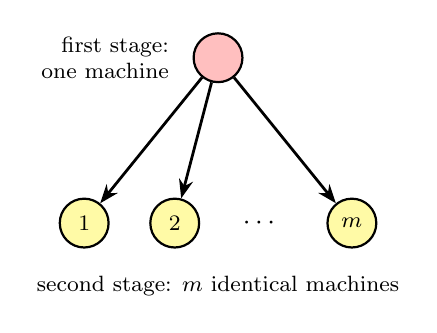
\begin{tikzpicture}[baseline=(current bounding box.center)]
\tikzset{mach/.style={circle,thick,draw,minimum size=0.62cm,inner sep=0pt,font=\footnotesize}}
% the shop: one first-stage machine feeding m identical second-stage machines
\node[mach,fill=red!25] (s) at (0,1.2) {};
\node[anchor=east,font=\footnotesize,align=right] at (-0.5,1.2) {first stage:\\one machine};
\node[mach,fill=yellow!35] (m1) at (-1.7,-0.9) {$1$};
\node[mach,fill=yellow!35] (m2) at (-0.55,-0.9) {$2$};
\node at (0.55,-0.9) {$\cdots$};
\node[mach,fill=yellow!35] (mm) at (1.7,-0.9) {$m$};
\foreach \t in {m1,m2,mm}
    \draw[-{Stealth[length=2.4mm]},line width=1pt] (s) -- (\t);
\node[font=\footnotesize] at (0,-1.7) {second stage: $m$ identical machines};
\end{tikzpicture}%
\hspace{1.4cm}%
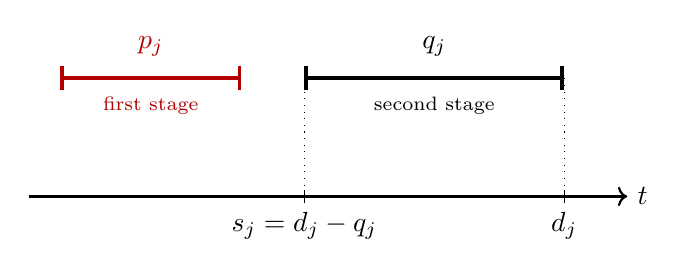
\begin{tikzpicture}[baseline=(current bounding box.center)]
\colorlet{prep}{red!70!black}
% the two operations of one job
\draw[->,thick] (-0.2,0) -- (7.4,0) node[right] {$t$};
\draw[|-|,line width=1.4pt,prep] (0.2,1.5) -- (2.5,1.5);
\node[prep] at (1.35,1.9) {$p_j$};
\node[prep,font=\scriptsize] at (1.35,1.15) {first stage};
\draw[|-|,line width=1.4pt] (3.3,1.5) -- (6.6,1.5);
\node at (4.95,1.9) {$q_j$};
\node[font=\scriptsize] at (4.95,1.15) {second stage};
\draw[dotted] (3.3,1.5) -- (3.3,0);
\draw[dotted] (6.6,1.5) -- (6.6,0);
\draw (3.3,0.08) -- (3.3,-0.08) node[below] {$s_j=d_j-q_j$};
\draw (6.6,0.08) -- (6.6,-0.08) node[below] {$d_j$};
\end{tikzpicture}

    \caption{A flexible flow shop with one first-stage machine and $m$ identical second-stage
    machines, and the two operations of a job $j$: the preprocessing, of length $p_j$, and the
    processing, which must occupy the interval $[s_j,d_j)$.}
    \label{fig:model}
\end{figure}

% lax begin Lax496464.EstOrder
Jobs are indexed in \emph{earliest-start-time order} (EST order), so that
$s_1\le\cdots\le s_n$; as in the paper, processing times are positive. The programs of
\Cref{sec:sweep,sec:smallq} also assume that the $2n$ endpoints $s_j,d_j$ are pairwise
distinct, which a rescaling achieves (\Cref{sec:sweep}).
% lax end

% lax begin Lax496464.Conditions
A set $\calZ\subseteq\calJ$ satisfies
\begin{itemize}
\item \emph{Condition 1} if it can be preprocessed in time:
  $\sum_{i\in\calZ,\,i\le j}p_i\le s_j$ for every $j\in\calZ$; and
\item \emph{Condition 2} if it can be scheduled on $m$ machines: $\calZ$ can be partitioned
  into $m$ classes, each without two jobs in conflict.
\end{itemize}
% lax end

% lax begin Lax496464.Feasibility
\begin{characterization}
A set $\calZ$ is feasible if and only if it satisfies Conditions 1 and 2. Condition 2 holds if
and only if at most $m$ jobs of $\calZ$ are running at any one instant.
\end{characterization}
% lax begin Lax496464Proofs.Section2.feasible_iff_conditions
The two stages decouple: the first-stage machine and the second-stage machines constrain
$\calZ$ separately, and schedules meeting the two conditions combine into one schedule of the
shop. The second sentence is the perfectness of interval graphs; it is what allows the tables
of \Cref{sec:sweep,sec:smallq} to be indexed by the jobs alive at an instant.
% lax end
% lax end

% lax begin Lax496464.Observation1
\begin{observation}\label{obs:EST}
A feasible set has a just-in-time schedule in which the first-stage operations are run in EST
order.
\end{observation}
% lax begin Lax496464Proofs.Section2.exists_est_schedule
By the exchange argument of Moore~\cite{Moore68}: if the first stage can meet the deadlines
$s_j$ in some order, it can meet them in order of nondecreasing $s_j$. Hence nothing is lost by
deciding which jobs to select without also deciding in which order to preprocess them.
\Cref{fig:est} shows a feasible set of five jobs.
% lax end
% lax end

\begin{figure}[tb]
    \centering
    % A feasible set of five jobs on two second-stage machines, with the first stage running
% the jobs in earliest-start-time order. Adapted from the slide "Key Observations".
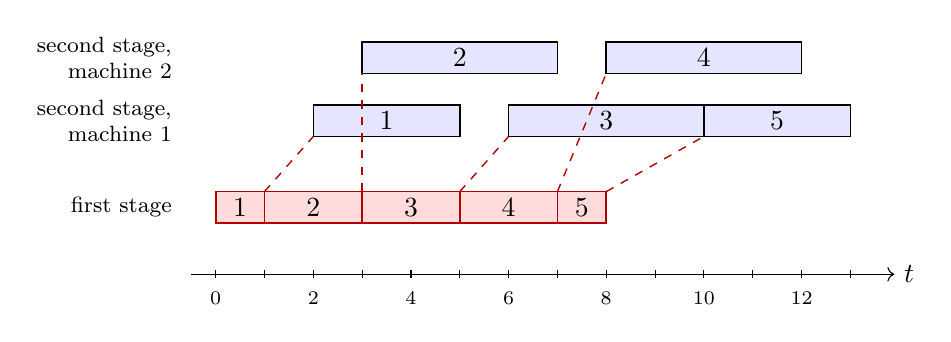
\begin{tikzpicture}[x=0.62cm,y=1cm]
\def\h{0.2}
\colorlet{prep}{red!70!black}
\tikzset{sop/.style={draw,fill=blue!10,line width=0.6pt},
         fop/.style={draw=prep,fill=red!14,line width=0.6pt}}

% the time axis
\draw[->] (-0.5,-0.55) -- (13.9,-0.55) node[right] {$t$};
\foreach \x in {0,1,...,13} \draw (\x,-0.5) -- (\x,-0.6);
\foreach \x in {0,2,4,6,8,10,12} \node[font=\scriptsize] at (\x,-0.85) {\x};

% row labels
\node[anchor=east,font=\footnotesize,align=right] at (-0.7,0.3) {first stage};
\node[anchor=east,font=\footnotesize,align=right] at (-0.7,1.4) {second stage,\\machine 1};
\node[anchor=east,font=\footnotesize,align=right] at (-0.7,2.2) {second stage,\\machine 2};

% second operations: job / start s_j / due date d_j / row
\foreach \j/\s/\d/\y in {1/2/5/1.4, 2/3/7/2.2, 3/6/10/1.4, 4/8/12/2.2, 5/10/13/1.4}
    \draw[sop] (\s,\y-\h) rectangle (\d,\y+\h) node[midway] {$\j$};

% first operations in earliest-start-time order, each ending by the start time s_j
\foreach \j/\a/\b/\s/\y in {1/0/1/2/1.4, 2/1/3/3/2.2, 3/3/5/6/1.4, 4/5/7/8/2.2, 5/7/8/10/1.4}
{
    \draw[fop] (\a,0.3-\h) rectangle (\b,0.3+\h) node[midway] {$\j$};
    \draw[dashed,prep,line width=0.5pt] (\b,0.3+\h) -- (\s,\y-\h);
}
\end{tikzpicture}

    \caption{A feasible set of five jobs on two second-stage machines. The first stage runs the
    jobs in EST order, and the preprocessing of job $j$ ends by $s_j$ (dashed). The jobs on
    each machine do not overlap.}
    \label{fig:est}
\end{figure}

% lax begin Lax496464.WordEncoding
An instance is given to a word RAM as a word of numbers: $n$, $m$, the $n$ preprocessing times,
the $n$ processing times, the $n$ due dates and the $n$ weights, in this order. In the decision
version the word ends with the threshold $W^*$.
% lax end
% lax begin Lax496464.BinaryEncoding
For \NP-hardness an instance is encoded as a binary word.
% lax end

% lax begin Lax496464.Problems
We consider the decision problem of whether there is a feasible set of weight at least $W^*$,
parameterized by the number $m$ of machines. The quantities $W$, $\omega$, $\qmax$ and $P$ that
appear in the running times are functions of the word. The bounds below are those of the paper
with a term $O(n\log n)$ added for putting the jobs into EST order, which the paper assumes
done and a program reading an arbitrary word has to pay for.
% lax end

\section{A Fixed Number of Machines}\label{sec:FixNumMachines}

% lax begin Lax496464.DynamicProgram
The jobs are considered from the last to the first. A set $X\subseteq\calJ$ of at most $m$
\emph{thresholds} describes the second-stage machines: a schedule is \emph{compatible} with
$X=\{x_1<\cdots<x_{|X|}\}$ if machine $i$ runs only jobs from $\{x_i,\ldots,n\}$ and the
machines $|X|+1,\ldots,m$ run none. The entry $T[X,W']$ of the table is the largest $P'$ such
that some feasible $\calZ$ of weight $W'$ compatible with $X$ can be preprocessed starting at
time $P'$; it is $-\infty$ if there is none and $+\infty$ if the empty set will do. For
$X\neq\emptyset$
let $j=\min X$, let $j_1=\min\{j^*\notin X: j^*>j\}$ and $j_2=\min\{j^*\notin X: s_{j^*}\ge
d_j\}$, and let $X_i=(X\setminus\{j\})\cup\{j_i\}$, or $X\setminus\{j\}$ if $j_i$ does not
exist (\Cref{fig:thresholds}). The table is filled by
\begin{equation}\label{eq:firstrec}
T[X,W']=\max\begin{cases}
T[X_1,W'],\\
\min\{T[X_2,W'-w_j],\,s_j\}-p_j.
\end{cases}
\end{equation}
% lax end

\begin{figure}[tb]
    \centering
    % The state of the dynamic program of Section 3: a set X of thresholds, and the sets X_1 and X_2
% that recursion (1) consults. Adapted from the slide "Dynamic Program".
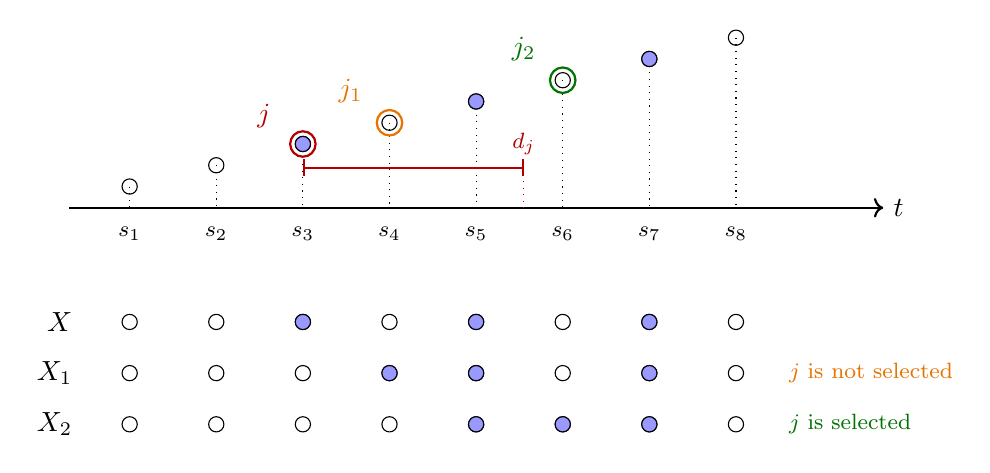
\begin{tikzpicture}[x=1.1cm,y=1cm]
\colorlet{prep}{red!70!black}
\colorlet{jone}{orange!90!black}
\colorlet{jtwo}{green!45!black}
\tikzset{dot/.style={draw,circle,inner sep=0pt,minimum size=5.5pt}}

% start times s_1, ..., s_8, in earliest-start-time order
\draw[->,thick] (0.3,0) -- (9.7,0) node[right] {$t$};
\foreach \i in {1,...,8}
{
    \pgfmathsetmacro{\yy}{0.27*\i}
    \draw[dotted] (\i,\yy) -- (\i,0);
    \node[font=\footnotesize] at (\i,-0.33) {$s_{\i}$};
    \node[dot] at (\i,\yy) {};
}
% the thresholds X = {3,5,7}; j = 3 is the smallest
\foreach \i in {3,5,7} \node[dot,fill=blue!40] at (\i,0.27*\i) {};
\draw[prep,thick] (3,0.27*3) circle (4.6pt);
\node[prep] at (2.55,0.27*3+0.35) {$j$};
% j_1 and j_2 are the smallest indices outside X above j, and with s >= d_j respectively
\draw[jone,thick] (4,0.27*4) circle (4.6pt);
\node[jone] at (3.55,0.27*4+0.4) {$j_1$};
\draw[jtwo,thick] (6,0.27*6) circle (4.6pt);
\node[jtwo] at (5.55,0.27*6+0.4) {$j_2$};
% the second operation of j
\draw[|-|,thick,prep] (3,0.27*3-0.3) -- (5.55,0.27*3-0.3);
\draw[dotted,prep] (5.55,0.27*3-0.3) -- (5.55,0);
\node[prep,font=\footnotesize] at (5.55,0.27*3+0.0) {$d_j$};

% the three threshold sets, one row each
\foreach \lab/\ysym/\members in {X/-1.45/{3,5,7}, X_1/-2.1/{4,5,7}, X_2/-2.75/{5,6,7}}
{
    \node[anchor=east] at (0.45,\ysym) {$\lab$};
    \foreach \i in {1,...,8} \node[dot] at (\i,\ysym) {};
    \foreach \i in \members \node[dot,fill=blue!40] at (\i,\ysym) {};
}
\node[anchor=west,font=\footnotesize,jone] at (8.5,-2.1) {$j$ is not selected};
\node[anchor=west,font=\footnotesize,jtwo] at (8.5,-2.75) {$j$ is selected};
\end{tikzpicture}

    \caption{The thresholds $X=\{3,5,7\}$ among eight jobs in EST order, with $j=3$. The set
    $X_1$ replaces $j$ by the smallest index $j_1=4$ outside $X$ above it; the set $X_2$
    replaces it by the smallest index $j_2=6$ outside $X$ whose start time is at least $d_j$.
    Recursion~\eqref{eq:firstrec} reads the table at $X_1$ if $j$ is not selected and at $X_2$
    if it is.}
    \label{fig:thresholds}
\end{figure}

% lax begin Lax496464.Lemma1
\begin{lemma}\label{lem:mainDP}
Recursion~\eqref{eq:firstrec} correctly computes $T[X,W']$ for every $X$ with $|X|\le m$ and
every $W'$.
\end{lemma}
% lax begin Lax496464Proofs.Section3.achievable_recursion
The recursion is formalized as an equivalence: a set of weight $W'$ compatible with $X$ can be
preprocessed from $P'$ exactly when a set of weight $W'$ compatible with $X_1$ can (job $j$ is
not selected), or $w_j\le W'$, $P'+p_j\le s_j$, and a set of weight $W'-w_j$ compatible with
$X_2$ can be preprocessed from $P'+p_j$ (job $j$ is selected and preprocessed first). The table
is the predicate ``can be preprocessed from $P'$'', which is downward closed in $P'$ and so
needs no infinite values. The hard direction takes a solution in which $j$ is not selected and
reassigns its jobs to the thresholds of $X_1$, an application of Hall's theorem.
% lax end
% lax end

% lax begin Lax496464.Theorem2
\setcounter{theorem}{1}
\begin{theorem}\label{thm:mainDP}
$\FF$ is solvable in $O(W\cdot n^m)$ time.
\end{theorem}
% lax begin Lax496464Proofs.Section3.achievable_readoff
The answer is read off the table at the $m$ smallest indices: a set of weight $W'$ compatible
with them that can be preprocessed from time $0$ is exactly a feasible set of weight $W'$.
% lax end
% lax begin Lax496464Proofs.Ram.D2Final.theorem2_time_proved
The formalized statement is a word RAM program, together with a constant $c$, that decides the
problem on every instance $x$ with threshold $W^*$, at every word length $w$ at which the input
and the table fit, within $c\,(W^*+1)(n+1)^m$ instructions plus the cost of sorting. The table
has $O(n^m)$ columns and $W+1$ rows, each entry computed from two earlier ones.
% lax end
% lax end

% lax begin Lax496464.Corollary1
\begin{corollary}\label{cor:unweighted}
$FF(1,1)\mid\mid\sum_jZ_j$ is solvable in $O(n^2)$ time.
\end{corollary}
% lax begin Lax496464Proofs.Ram.Corollary1Prog.corollary1_time_proved
This is \Cref{thm:mainDP} with $m=1$ and $W=n$.
% lax end
% lax end

% lax begin Lax496464.Corollary2
\begin{corollary}\label{cor:P}
$\FF$ is solvable in $O(P\cdot n^m)$ time, where $P=\sum_jp_j$.
\end{corollary}
% lax begin Lax496464Proofs.Ram.D4Final.corollary2_time_proved
The same table is read the other way round: it stores for each instant $P'\in\{0,\ldots,P\}$ the
largest weight attainable, by the recursion $T[X,P']=\max\{T[X_1,P'],\,T[X_2,P'+p_j]+w_j\}$,
where the second term is $-\infty$ if $P'+p_j>s_j$.
% lax end
% lax end

\section{A Program for Small $\omega$}\label{sec:sweep}

% lax begin Lax496464.Normalization
Setting $d_j'=(n+1)d_j+j$, $q_j'=(n+1)q_j$ and $p_j'=(n+1)p_j$ gives an equivalent instance with
pairwise distinct endpoints: it has the same feasible sets, with the same weights, and it
preserves the EST order.
% lax begin Lax496464Proofs.Section4.scale_feasible_iff
The content is that the rescaling creates no conflict where there was none and destroys none
where there was one.
% lax end
% lax end

% lax begin Lax496464.Sweep
Let $t_1<\cdots<t_{2n}$ be the endpoints and $X_i=\{j: s_j\le t_i<d_j\}$ the set of jobs whose
second operation contains $t_i$; so $\omega=\max_i|X_i|$. Let $\calJ_i=\bigcup_{\ell\le i}X_\ell$.
A feasible $\calZ\subseteq\calJ_i$ is \emph{compatible} with $X\subseteq X_i$ if
$\calZ\cap X_i=X$, and
\[
T_i[X,W']\;=\;\text{the least }p(\calZ)\text{ over feasible }\calZ\subseteq\calJ_i
\text{ of weight }W'\text{ compatible with }X.
\]
Since $X\subseteq X_i$ has at most $\omega$ members, each table has $W\cdot2^{\omega}$ entries.
If $t_i=s_j$, then
\begin{equation}\label{eq:startrec}
T_i[X,W']=\begin{cases}
T_{i-1}[X,W'] & j\notin X,\\
T_{i-1}[X\setminus\{j\},W'-w_j]+p_j & j\in X\text{ and this is at most }s_j,\\
\infty & \text{otherwise,}
\end{cases}
\end{equation}
and if $t_i=d_j$, then
\begin{equation}\label{eq:duerec}
T_i[X,W']=\begin{cases}
T_{i-1}[X,W'] & |X|=m,\\
\min\{T_{i-1}[X\cup\{j\},W'],\,T_{i-1}[X,W']\} & |X|<m.
\end{cases}
\end{equation}
% lax end

% lax begin Lax496464.Lemma2
\begin{lemma}\label{lem:2^w}
Recursions~\eqref{eq:startrec} and~\eqref{eq:duerec} correctly compute $T_i[X,W']$ for every
$i$, every $X\subseteq X_i$ and every $W'$.
\end{lemma}
% lax begin Lax496464Proofs.Section4.exists_reachable_iff
Both equations are formalized as equivalences, so each says at once that the recursion invents
no entry and loses none. Past the last start time the table answers the question: some state
carries weight $W'$ exactly when a feasible set of weight $W'$ exists.
% lax end
% lax end

\section{A Program for Small $\qmax$}\label{sec:smallq}

% lax begin Lax496464.Profile
The second program sweeps the jobs in EST order and carries, instead of the selected jobs alive
at $s_j$, only their \emph{profile}: the vector $\vecx\in\{0,\ldots,m\}^{\qmax}$ whose $i$th
entry is the number of machines that complete their last selected job at $s_j+i$, equivalently
the number of selected jobs due at $s_j+i$. Stepping from $s_{j-1}$ to $s_j$ moves the
reference point by $\delta_j=s_j-s_{j-1}$, so a profile at $s_{j-1}$ becomes a profile at $s_j$
shifted by $\delta_j$; let $\vecx[\delta]$ be the set of vectors that shift to $\vecx$, and
$\vecx^{(q)}$ the vector with entry $q$ decreased by one. The table
$T_j[\vecx,W']$ is the least $p(\calZ)$ over feasible selections $\calZ\subseteq\{1,\ldots,j\}$
of weight $W'$ whose profile at $s_j$ is $\vecx$, and
\begin{equation}\label{eq:lastrec}
T_j[\vecx,W']=\min\begin{cases}
\min_{\vec y\in\vecx[\delta_j]}T_{j-1}[\vec y,W'],\\
\min_{\vec y\in\vecx^{(q_j)}[\delta_j]}\;\begin{cases}
T_{j-1}[\vec y,W'-w_j]+p_j & \text{if this is at most }s_j,\\
\infty & \text{otherwise.}\end{cases}
\end{cases}
\end{equation}
The first case passes job $j$ over, the second selects it (\Cref{fig:profile}).
% lax end

\begin{figure}[tb]
    \centering
    % The dynamic program of Section 5 visualized: Figure 1 of the paper (EJOR), unchanged.
% A set Z of jobs in three reference frames, with the profiles x at s_j and y at s_{j-1}.
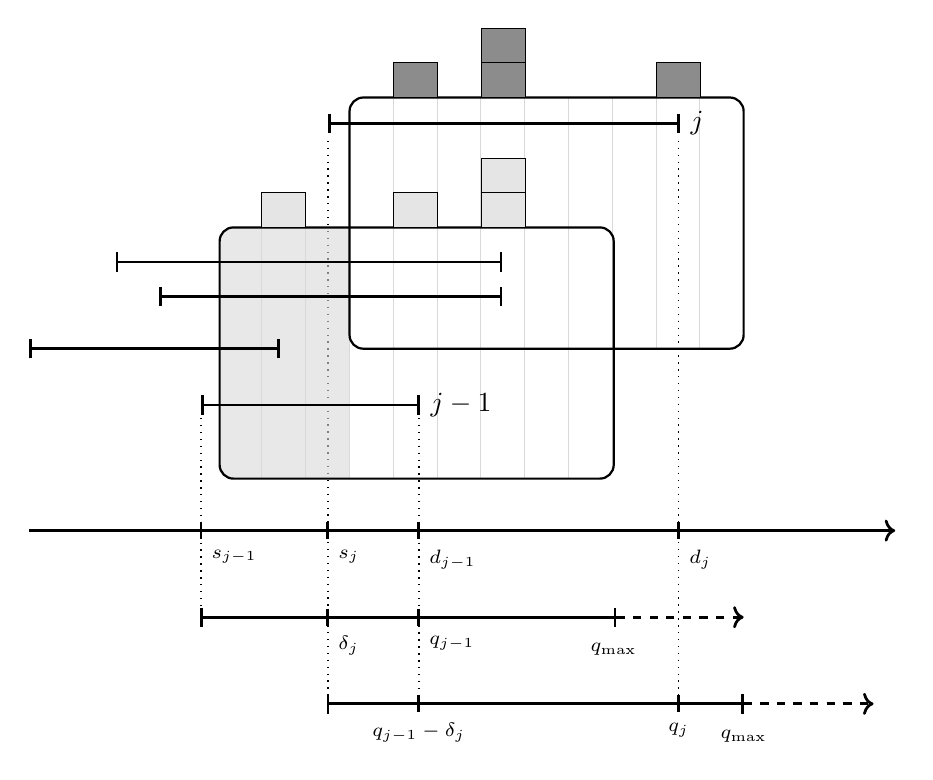
\begin{tikzpicture}[scale=1.1,yscale=1]

% Axis and ticks
\draw[line width=1, ->]
(0, -1) -- (10 , -1) node[] {};
\draw[line width=1, |-]
(3.5-1.526, -2) -- (3.5-1.5+4.75 , -2) node[] {};
\draw[line width=1,dashed, <-|]
 (3.5+4.75 , -2) -- (3.5-1.5+4.75, -2) node[] {};
 \draw[line width=1,dashed, ->]
 (3.5+4.75 , -3) -- (3.5+4.75+1.5, -3) node[] {};
\draw[line width=1, |-|]
(3.435, -3) -- (3.5+4.75, -3) node[below] {};
\node at (3.5+4.75, -3-0.375) {\scriptsize$q_{\max}$};
\node at (3.5-1.5+4.75, -2-0.375) {\scriptsize$q_{\max}$};

% }



\draw[line width=.5,dotted, -] (3.45, 3.5) -- (3.45, -3.1) node[below] {};
\draw[line width=1., -] (3.45, -.9) -- (3.45, -1.1) node[below right] {\scriptsize$s_{j}$};
\draw[line width=1., -] ((7.5, -.9) -- ((7.5, -1.1) node[below right] {\scriptsize$d_{j}$};
\draw[line width=1., -] ((6-1.5, -.9) -- ((6-1.5, -1.1) node[below right] {\scriptsize$d_{j-1}$};

\draw[line width=.5,dotted, -] (7.5, 3.5) -- (7.5, -3) node[below] {};
\draw[line width=1., -] (7.5, -2.9) -- (7.5, -3.1) node[below] {\scriptsize$q_{j}$};
% \draw[line width=1., -] (7.5, -1.9) -- (7.5, -2.1) node[below right] {\scriptsize$\delta_j+q_{j}$};


% Left gray half (manually shaded)
% Fill left half in gray
\fill[gray!30,opacity=.6]
  (2.0+0.2,-0.325) -- 
  (2.05+0.2,-0.35) -- 
  (2.1+0.2,-0.4) -- 
  (3.7,-0.4) -- 
  (3.7,2.5) -- 
  (2.1+0.2,2.5) -- 
  (2.0+0.2,2.4) -- 
  (2.0+0.2,2.5) -- 
  cycle;

% Histogram parameters
\def\xstart{3.5+0.2}
\def\xend{8.25}
\def\nbars{10}
\pgfmathsetmacro{\width}{(\xend - \xstart)/\nbars}



% Define rectangle corners
\def\xstart{2.2}
\def\xend{6.75}
\def\ystart{-0.4}
\def\yend{2.5}

% Number of vertical lines
\def\nlines{8}
% Draw vertical lines inside the rectangle
\pgfmathsetmacro{\spacing}{(\xend - \xstart)/(\nlines + 1)}
\foreach \i in {1,...,\nlines} {
    \pgfmathsetmacro{\x}{\xstart + \i * \spacing}
    \draw[thin,gray!30] (\x-0.017,\ystart) -- (\x-0.017,\yend);
}


% Define rectangle corners
\def\xstart{3.7}  % 3.5 + 0.2
\def\xend{8.25}
\def\ystart{1.1}
\def\yend{4.0}
% Number of vertical lines
\def\nlines{8}

\pgfmathsetmacro{\spacing}{(\xend - \xstart)/(\nlines + 1)}
\foreach \i in {1,...,\nlines} {
    \pgfmathsetmacro{\x}{\xstart + \i * \spacing}
    \draw[thin,gray!30] (\x,\ystart) -- (\x,\yend);
}

% Draw Rects
\draw[rounded corners=5pt, thick] (2.2,-0.4) rectangle (6.75,2.5);
\draw[rounded corners=5pt, thick] (3.5+0.2,1.1) rectangle (8.25,4.);


\draw[line width=.5,dotted, -] (1.985, .3) -- (1.985, -2.1) node[below] {};
\draw[line width=1., -] (1.985, -.9) -- (1.985, -1.1) node[below right] {\scriptsize$s_{j-1}$};


\draw[line width=.5,dotted, -] (6-1.5, .3) -- (6-1.5, -3) node[below] {};
\draw[line width=1., -] (6-1.5, -2.9) -- (6-1.5, -3.1) node[below] {\scriptsize$q_{j-1}-\delta_j$};
\draw[line width=1., -] (6-1.5, -1.9) -- (6-1.5, -2.1) node[below right] {\scriptsize$q_{j-1}$};


\draw[line width=1., -] (3.45, -1.9) -- (3.45, -2.1) node[below right] {\scriptsize$\delta_{j}$};



% jobs j and j-1
\draw[|-|,line width=1.,opacity=1.]
        (3.45 , 3.7) -- (7.5+.015, 3.7) node[right] {$j$};
\draw[|-|,line width=1.,opacity=1.]
        (1.985 , .45) -- (6-1.5+.015, .45) node[right] {$j-1$};

% The rest of the ints

        
\draw[|-|,line width=1.,opacity=1.]
        (3.6-1.5-.35-.25 , 1.7) -- (6-1.5+.015+0.95, 1.7) node[] {};
\draw[|-|,line width=1.,opacity=1.]
        (3.6-1.5-.35-.75 , 2.1) -- (6-1.5+.015+0.95, 2.1) node[] {};

\draw[|-|,
% gray!90,
line width=1.,opacity=1.]
        (.0 , 1.1) -- (2.9, 1.1) node[] {};



% The histogram

% q_j
\draw[fill=gray!90] (7.24,4.) rectangle ++(\width+.015,.4);

% middle
\draw[fill=gray!90] (7.24-4*\width-.04,4.4) rectangle ++(\width+.015,.4);
\draw[fill=gray!90] (7.24-4*\width-.04,4.) rectangle ++(\width+.015,.4);

% q_j-1
\draw[fill=gray!90] (7.24-6*\width-.0625,4.) rectangle ++(\width+.015,.4);

% previous
% \draw[fill=gray!30] (7.24-9*\width-.0625,4.) rectangle ++(\width+.015,.4);
\draw[fill=gray!20] (7.24-9*\width-.1,2.5) rectangle ++(\width+.015,.4);


% middle
\draw[fill=gray!20] (7.24-4*\width-.04,2.9) rectangle ++(\width+.015,.4);
\draw[fill=gray!20] (7.24-4*\width-.04,2.5) rectangle ++(\width+.015,.4);

% q_j-1
\draw[fill=gray!20] (7.24-6*\width-.0625,2.5) rectangle ++(\width+.015,.4);

\end{tikzpicture}

    \caption{The dynamic program visualized. A set~$\calZ$ of jobs is shown in three reference
    frames: the top axis is the main line beginning at $0$, the middle axis the reference of $j-1$
    beginning at $s_{j-1}$, and the bottom one the reference of $j$ beginning at $s_j$. The boxes
    above each sliding window represent the number of machines that complete processing their last
    job at that time. In the example, assuming that all jobs can be preprocessed in time, $\calZ$
    has profile $\vecx$ at $s_j$ and the solution $\calZ\setminus\{j\}$ has profile $\vec y$ at
    $s_{j-1}$, with $\qmax=9$, $\delta_j=3$, $\vecx=(0,1,0,2,0,0,0,1,0)$ and
    $\vec y=(0,1,0,0,1,0,2,0,0)$. Observe that $\vec y\in\vecx^{(q_j)}[\delta_j]$, and also
    $\vec y\in\vecx[\delta_j]$; in the example this set is $\vecx^{(8)}[3]$.}
    \label{fig:profile}
\end{figure}

% lax begin Lax496464.Lemma3
\begin{lemma}\label{lem:qmax}
Recursion~\eqref{eq:lastrec} computes the table of due-date profiles.
\end{lemma}
% lax begin Lax496464Proofs.Section5.exists_reachableProfile_iff
The formalization maintains the invariant in the following form: an entry
$T_j[\vecx,W']\le P'$ is witnessed by a feasible selection of weight $W'$ and preprocessing cost
at most $P'$ whose profile is \emph{at most} $\vecx$ coordinatewise, and every feasible
selection is still derived with its exact profile. A vector that overstates the profile only
overstates how many machines are busy, so the capacity test rejects more rather than less, and
the optimum read off at the end is exact. Small examples, one job on two machines and two jobs
on one machine, show that the entries do not carry the exact profile, which is why the weaker form
is the one that is proved.
% lax end
% lax end

% lax begin Lax496464.Theorem3
\setcounter{theorem}{2}
\begin{theorem}\label{thm:secondaryDPs}
$\FF$ can be solved in
\begin{itemize}
\item $O(W\cdot2^{\omega}\cdot n)$ time, where $\omega$ is the largest number of jobs whose
  second operations contain a common instant, and
\item $O(W\cdot m^{\qmax}\cdot n)$ time, where $\qmax=\max_jq_j$.
\end{itemize}
\end{theorem}
% lax begin Lax496464Proofs.Ram.W3Final.theorem3_width_time_proved
The first bullet is a word RAM program that carries the table of
recursions~\eqref{eq:startrec} and~\eqref{eq:duerec} through the $2n$ endpoints.
% lax end
% lax begin Lax496464Proofs.Ram.Q3Final.theorem3_qmax_time_proved
The second is a program that carries the profiles of recursion~\eqref{eq:lastrec}, one
marginalization pass per job. Each bound has its own fitting condition, for its own table, and
neither involves $m$ in the exponent.
% lax end
% lax end

\section{Uniform Preprocessing Times}\label{sec:uniform}

% lax begin Lax496464.ProperInstances
In this section $p_j=p$ for all jobs. An instance is \emph{proper} if no interval $[s_i,d_i)$ is
contained in another; the EST order and the order by due dates then coincide.
% lax end

% lax begin Lax496464.Greedy
For unit weights the jobs are taken in EST order, maintaining a set $\calZ$ of selected jobs. At
job $j$, if $s_j\ge(|\calZ|+1)p$ and fewer than $m$ jobs of $\calZ$ are alive at $s_j$, then $j$
joins $\calZ$; otherwise one job of $\calZ\cup\{j\}$ with the largest due date is dropped. The
set kept is compared to others through a \emph{domination} order: $\calZ'$ dominates $\calZ''$
if it has more jobs, or the same number and, for every $i$, its $i$th largest due date is not
greater than the $i$th largest due date of $\calZ''$.
% lax end

% lax begin Lax496464.Lemma4
\begin{lemma}\label{lem:greedy}
After the greedy has considered the first $j$ jobs, its set is feasible and dominates every
feasible set of jobs among them. Consequently it ends with a feasible set of largest
cardinality.
\end{lemma}
% lax begin Lax496464Proofs.Section6.greedy_dominating
The proof is by induction on $j$ over the three cases of the step: the job joins the set, or the
first stage cannot preprocess one more job, or $m$ selected jobs are alive at $s_j$. In the last
two the greedy keeps the set of the previous step without its latest due date.
% lax end
% lax end

% lax begin Lax496464.IntegerProgram
For weights, on a proper instance, a set is feasible exactly when its indicator vector
$\mathbf x\in\{0,1\}^n$ satisfies, for every job $j$,
\begin{equation}\label{eq:ilp}
\sum_{i\le j}x_i\le\lfloor s_j/p\rfloor,\qquad\sum_{i:\,s_i\le s_j<d_i}x_i\le m.
\end{equation}
The first inequality is Condition~1, since with equal preprocessing times the time spent is the
number of jobs run, and the second is Condition~2 in its depth form, tested at the start times.
The scheduling problem is therefore the integer program that maximizes $\sum_jw_jx_j$ subject
to~\eqref{eq:ilp}.
% lax end

% lax begin Lax496464.ConsecutiveOnes
A matrix has the \emph{consecutive ones property} if the ones in each row are consecutive. Such
a matrix is totally unimodular~\cite{FG65}: every square submatrix has determinant $0$, $1$ or
$-1$.
% lax begin Lax496464Proofs.Section6.isTotallyUnimodular
This theorem of Fulkerson and Gross is proved rather than assumed.
% lax end
% lax end

% lax begin Lax496464.Lemma5
\begin{lemma}\label{lem:ilp}
On a proper instance the constraint matrix of~\eqref{eq:ilp} has the consecutive ones
property, and hence is totally unimodular.
\end{lemma}
% lax begin Lax496464Proofs.Section6.lemma5
The jobs alive at any one instant form a consecutive block of the EST order, so the first family
of rows consists of prefixes and the second of blocks. That the feasible solutions of the program
are exactly the feasible sets holds on every instance with equal positive preprocessing times,
proper or not.
% lax end
% lax end

% lax begin Lax496464.Corollary3
\begin{corollary}\label{cor:uniform}
$FF(1,m)\mid p_j=p\mid\sum_jw_jZ_j$ is solvable in $O(n^{m+1})$ time.
\end{corollary}
% lax begin Lax496464Proofs.Ram.D5Final.corollary3_time_proved
With equal preprocessing times the instant a partial solution has spent is determined by the
number of jobs it has selected, so the dual table of \Cref{cor:P} takes only $n+1$ values of
$P'$.
% lax end
% lax end

% lax begin Lax496464.Theorem4
\setcounter{theorem}{3}
\begin{theorem}\label{thm:Uniform}
$FF(1,m)\mid p_j=p\mid\sum_jw_jZ_j$ is solvable in $O(n\log n)$ time when $w_j=1$ for all
jobs, and in $O(n^{2.5}\cdot\max\{\log W,\log P\})$ time on proper instances.
\end{theorem}
% lax begin Lax496464Proofs.Ram.T4Final.theorem4_greedy_time_proved
The first part is the greedy, whose cost beyond sorting is one pass. The formalized part of the
second is the integer program, its correctness and the total unimodularity of its matrix
(\Cref{lem:ilp}); that a linear program with a totally unimodular matrix has an integral
optimum~\cite{HK56} and is solved in polynomial time are cited.
% lax end
% lax end

\section{Approximation Schemes}\label{sec:approx}

% lax begin Lax496464.Fptas
Let $\varepsilon>0$ and $k=\varepsilon\wmax/n$, and round the weights to $w_j^*=\lceil
w_j/k\rceil$. Let $\calZ^*$ be an optimal solution for $w^*$ and $\calZ$ one for $w$. The
optimum is at least $\wmax$, so
\begin{equation}\label{eq:rounding}
w(\calZ^*)\;\ge\;k\,w^*(\calZ^*)-kn\;\ge\;w(\calZ)-\varepsilon\wmax\;\ge\;(1-\varepsilon)\,w(\calZ).
\end{equation}
An \emph{approximation scheme} is a program that is handed an instance and an integer $e$ and
returns a number that a feasible set reaches and that is within a factor $1-1/e$ of the optimum.
% lax end

% lax begin Lax496464.Theorem5
\setcounter{theorem}{4}
\begin{theorem}\label{thm:fptas}
$\FF$ admits a fully polynomial-time approximation scheme when $m=O(1)$, or $\qmax=O(1)$, or
$\omega=O(\log n)$.
\end{theorem}
% lax begin Lax496464Proofs.Section7.rescale_approx
The rounding argument~\eqref{eq:rounding} is proved on its own. It assumes that there is a
machine to run a job on and that $p_j\le s_j$ for every job, jobs failing which are discarded.
% lax end
% lax begin Lax496464Proofs.F5MFinal.theorem5_byMachines_proved
After rounding, the threshold to search is of order $n^2e$, so each of the three exact programs
becomes a scheme whose running time is that of the program with $W$ replaced by $n^2e$: the
table of \Cref{thm:mainDP} gives the scheme for $m=O(1)$,
% lax end
% lax begin Lax496464Proofs.F5WFinal.theorem5_byWidth_proved
the endpoint sweep gives the scheme for $\omega=O(\log n)$,
% lax end
% lax begin Lax496464Proofs.F5QConclude.theorem5_byQmax_proved
and the profile sweep gives the scheme for $\qmax=O(1)$.
% lax end
% lax end

\section{Hardness}\label{sec:hardness}

% lax begin Lax496464.HittingSet
\begin{definition}[\HS]
We are given a family $\mathcal F=\{F_1,\ldots,F_m\}$ of subsets of a universe
$U=\{1,\ldots,n\}$ and an integer $k$, and are asked whether there is a set $H\subseteq U$ with
$|H|=k$ that meets every $F\in\mathcal F$. The parameter is $k$.
\end{definition}
\HS\ is \NP-hard~\cite{GJ79} (problem SP8) and \Wtwo-hard for $k$~\cite{DF99}. The instances
considered here have $2\le k\le n$.
% lax end

% lax begin Lax496464.NPHardness
A problem is \emph{\NP-hard} if every language in \NP\ has a polynomial-time many-one reduction
to it, and \emph{strongly \NP-hard} if the reduction can be chosen to emit instances whose
numbers are bounded by a fixed polynomial in the length of the input.
% lax end
% lax begin Lax496464.ParameterizedComplexity
An \emph{fpt-reduction} is a map on words that preserves and reflects yes-instances, raises the
parameter by at most a function of it, and is computed by a word RAM program within
$c\,g(k)(|x|+1)^c$ instructions.
% lax end
% lax begin Lax496464.W2Hardness
A parameterized problem is \Wtwo-hard if \HS, parameterized by $k$, fpt-reduces to it.
% lax end

% lax begin Lax496464.Construction
\begin{construction}\label{const:hardness}
Let $(U,\mathcal F,k)$ be an instance of \HS\ with $2\le k\le n$. Let $R=k(n-1)+2$ be the number
of \emph{segments} and $Q=(k-1)(n+1)$. We build an instance of $FF(1,k)\mid\mid\sum_jZ_j$. The
time axis is divided into $R$ segments of $m$ \emph{epochs} each, one epoch per set of the
family. For $r\in\{0,\ldots,R-1\}$ and $j\in\{1,\ldots,m\}$ let $g(r,j)=rm+j$ and
$G(r,j)=g(r,j)^2\,Q$; the epoch $T^r_j$ is the interval from $G(r,j)$ to the start of the next
epoch, of length $(2g(r,j)+1)Q$. The jobs of epoch $T^r_j$, all of weight $1$, are
\begin{itemize}
\item for each $i\in F_j$ a \emph{selection job} $S^r_{i,j}$ with preprocessing time $0$,
  processing time $(2g(r,j)+1)Q$ and due date $G(r,j)+(2g(r,j)+1)Q+i$;
\item for each $i\in U$ a \emph{dummy job} $A^r_{i,j}$ with preprocessing time
  $g(r,j)(n+1)$, processing time $g(r,j)Q$ and due date $G(r,j)+g(r,j)Q+i$; and
\item for each $i\in U$ a \emph{dummy job} $B^r_{i,j}$ with preprocessing time
  $g(r,j)(n+1)$, processing time $(g(r,j)+1)Q$ and due date $G(r,j)+(2g(r,j)+1)Q+i$.
\end{itemize}
The target is $R\cdot m\cdot(2k-1)$ just-in-time jobs.
\end{construction}
Thus $A^r_{i,j}$ ends when $B^r_{i,j}$ starts, and $B^r_{i,j}$ ends when the next epoch starts,
up to the offset $i$; see \Cref{fig:hardness}. Two details are done slightly differently than
in~\cite{HHISS26}: the number of segments is $k(n-1)+2$, which is what the pigeonhole argument
below uses, and the construction is stated for $2\le k\le n$, the range in which $Q$ is
positive and a hitting set of size $k$ can exist. The elements are numbered from $0$ in the
formalization, with $i+1$ in place of $i$ in the due dates.
% lax end

\begin{figure}[tb]
    \centering
    % The first segment of the shop built from the Hitting Set instance U = {1,2,3}, F_1 = {2,3},
% F_2 = {1,2}, F_3 = {1,3}, k = 2, drawn to scale: the unit is Q = (k-1)(n+1) = 4, the three epochs
% have lengths 3Q, 5Q and 7Q, and the jobs of element i are shifted by i = Q * (i/4).
% Adapted from the construction figure of the paper.
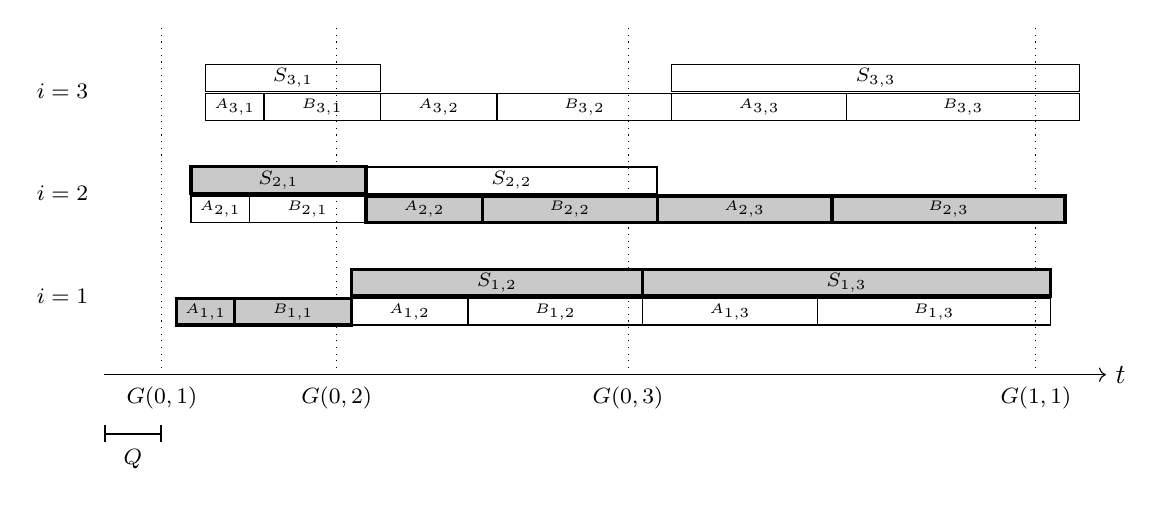
\begin{tikzpicture}[x=0.74cm,y=1cm]
\def\h{0.17}
\colorlet{sel}{gray!42}
\tikzset{job/.style={draw,line width=0.5pt},
         chosen/.style={draw,fill=sel,line width=1.2pt}}

% the epoch boundaries G(0,1) = Q, G(0,2) = 4Q, G(0,3) = 9Q, G(1,1) = 16Q
\foreach \g/\lab in {1/{G(0,1)}, 4/{G(0,2)}, 9/{G(0,3)}, 16/{G(1,1)}}
{
    \draw[dotted] (\g,-0.55) -- (\g,3.85);
    \node[font=\footnotesize] at (\g,-0.85) {$\lab$};
}
\draw[->] (0,-0.55) -- (17.2,-0.55) node[right] {$t$};
\draw[|-|,line width=0.8pt] (0,-1.3) -- (1,-1.3);
\node[font=\footnotesize] at (0.5,-1.62) {$Q$};

% rows: element i = 1, 2, 3 (bottom to top); a selection job S_{i,j} lies above two dummies A, B
\foreach \i in {1,2,3}
{
    \pgfmathsetmacro{\yD}{(\i-1)*1.3+0.25}
    \pgfmathsetmacro{\yS}{(\i-1)*1.3+0.62}
    \pgfmathsetmacro{\sh}{\i/4}
    \node[anchor=east,font=\footnotesize] at (-0.1,\yD+0.2) {$i=\i$};
    \foreach \j/\g/\gn in {1/1/4, 2/4/9, 3/9/16}
    {
        \pgfmathsetmacro{\xa}{\g+\sh}
        \pgfmathsetmacro{\xm}{\g+\j+\sh}
        \pgfmathsetmacro{\xb}{\gn+\sh}
        \draw[job] (\xa,\yD-\h) rectangle (\xm,\yD+\h) node[midway,font=\tiny] {$A_{\i,\j}$};
        \draw[job] (\xm,\yD-\h) rectangle (\xb,\yD+\h) node[midway,font=\tiny] {$B_{\i,\j}$};
    }
}
% selection jobs: S_{i,j} exists when i is in F_j
\foreach \i/\j/\g/\gn in {1/2/4/9, 1/3/9/16, 2/1/1/4, 2/2/4/9, 3/1/1/4, 3/3/9/16}
{
    \pgfmathsetmacro{\yS}{(\i-1)*1.3+0.62}
    \pgfmathsetmacro{\sh}{\i/4}
    \draw[job] (\g+\sh,\yS-\h) rectangle (\gn+\sh,\yS+\h) node[midway,font=\scriptsize] {$S_{\i,\j}$};
}
% the schedule of the hitting set H = {1,2}, in gray
\foreach \i/\j/\g/\gn in {2/1/1/4, 1/2/4/9, 1/3/9/16}
{
    \pgfmathsetmacro{\yS}{(\i-1)*1.3+0.62}
    \pgfmathsetmacro{\sh}{\i/4}
    \draw[chosen] (\g+\sh,\yS-\h) rectangle (\gn+\sh,\yS+\h) node[midway,font=\scriptsize] {$S_{\i,\j}$};
}
\foreach \i/\j/\g/\gm/\gn in {1/1/1/2/4, 2/2/4/6/9, 2/3/9/12/16}
{
    \pgfmathsetmacro{\yD}{(\i-1)*1.3+0.25}
    \pgfmathsetmacro{\sh}{\i/4}
    \draw[chosen] (\g+\sh,\yD-\h) rectangle (\gm+\sh,\yD+\h) node[midway,font=\tiny] {$A_{\i,\j}$};
    \draw[chosen] (\gm+\sh,\yD-\h) rectangle (\gn+\sh,\yD+\h) node[midway,font=\tiny] {$B_{\i,\j}$};
}
\end{tikzpicture}

    \caption{\Cref{const:hardness} for $U=\{1,2,3\}$, $F_1=\{2,3\}$, $F_2=\{1,2\}$,
    $F_3=\{1,3\}$ and $k=2$, drawn to scale; only the first segment is shown. Each row holds the
    jobs of one element $i$, shifted by $i$, with the selection jobs above the dummy pairs. Gray
    jobs form the schedule for the hitting set $H=\{1,2\}$: in each epoch one machine runs a
    selection job and the other runs the two dummy jobs of its element.}
    \label{fig:hardness}
\end{figure}

% lax begin Lax496464.Theorem1
\setcounter{theorem}{0}
\begin{theorem}\label{thm:NP-hard}
$\FFu$ is strongly \NP-hard.
\end{theorem}
% lax begin Lax496464Proofs.Section8.construct_correct
The family has a hitting set of size $k$ if and only if the instance of \Cref{const:hardness}
has $R\cdot m\cdot(2k-1)$ jobs that can be completed just in time. Given a hitting set $H$, let
$i_j$ be the least element of $F_j\cap H$. In every epoch the machine of $i_j$ runs the
selection job $S^r_{i_j,j}$, and the machine of every other element of $H$ runs its two dummy
jobs; the preprocessing of the $k-1$ dummy pairs of an epoch takes exactly $2g(r,j)Q$ and fits
before the epoch starts. Conversely, the preprocessing budget of an epoch admits at most
$2(k-1)$ dummy jobs, so a solution of the target size holds exactly one selection job and
$2(k-1)$ dummies in every epoch. The offsets $i$ make the element a machine is responsible for
nondecreasing from one segment to the next, and it takes values in $\{1,\ldots,n\}$, so it
changes at most $n-1$ times. With more than $k(n-1)$ gaps between segments some gap sees no
change on any machine, and the $k$ elements of that segment hit every set.
% lax end
% lax begin Lax496464Proofs.Ram.Theorem1Final.stronglyNPHard_hasWeight_proved
The numbers of the instance are polynomial in $n$, $m$ and $k$, hence in the length of the
\HS\ instance, so the hardness is strong: no pseudo-polynomial algorithm exists unless
$\mathrm P=\NP$.
% lax end
% lax end

% lax begin Lax496464.Corollary4
\begin{corollary}\label{cor:W2}
$\FFu$ is \Wtwo-hard with respect to the number $m$ of machines.
\end{corollary}
% lax begin Lax496464Proofs.Corollary4.w2Hard_byMachines
The shop of \Cref{const:hardness} has exactly $k$ machines, so the construction is an
fpt-reduction from \HS. Hence an algorithm with running time $f(m)\cdot n^{O(1)}$ would give
$\FPT=\Wtwo$.
% lax end
% lax end

% lax begin Lax496464.HittingSetFromSat
\Cref{thm:NP-hard} rests on the \NP-hardness of \HS, which is proved here as well, by the
standard reduction from satisfiability. A CNF formula $F$ on variables $x_0,\ldots,x_{V-1}$
becomes the instance on the universe $\{0,\ldots,2V-1\}$ in which $2i$ stands for the literal
$x_i$ and $2i+1$ for $\bar x_i$. The family has one set $\{2i,2i+1\}$ for each variable and one
set for each clause, holding the elements of its literals, and $k=V$. A hitting set of size $V$
meets each of the $V$ disjoint pairs in exactly one element, so it is a truth assignment, and
it meets the set of a clause exactly when the assignment satisfies the clause. This is the
composition of Karp's reductions~\cite{Karp72} from satisfiability to Clique and from Clique to
Node Cover, read on the literals.
% lax end

% lax begin Lax496464.HittingSetHardness
\begin{karp}\label{thm:hs}
Every language in \NP\ reduces to \HS\ in polynomial time, by a reduction whose output
instances are of polynomial size and satisfy $2\le k\le n$.
\end{karp}
% lax begin Lax496464Proofs.HittingSet.Correct.fromSat_correct
A formula is satisfiable exactly when its instance has a hitting set of the required size.
% lax end
% lax begin Lax496464Proofs.HittingSet.Final.fromSat_polyTime
The reduction on words decodes a formula, builds the instance and encodes it; it is a word RAM
program, and
% lax begin lax-759944
its polynomial running time is transferred to a Turing machine by the equivalence of the two
machine models.
% lax end
% lax end
% lax begin lax-429075
Composed with the Cook--Levin theorem of the archive, this makes every language in \NP\ reduce to
\HS.
% lax end
% lax begin Lax496464Proofs.HittingSet.Hardness.hittingSet_npHard
The two restrictions on $k$ cost nothing: a hitting set of size exactly $k$ cannot exist once
$k$ exceeds the universe, and for $k<2$ an instance is padded with a fresh element and the
singleton containing it, which forces that element into every hitting set and raises $k$ by one.
The universe of an emitted instance is no larger than $4+m+\sum_j|F_j|$, so the shop of
\Cref{const:hardness}, which has more than $n^2$ jobs, can be written in time polynomial in the
word that presents the instance.
% lax end
% lax end

\begin{thebibliography}{9}
\bibitem{CL95}
M.~C. Carlisle and E.~L. Lloyd.
\newblock On the $k$-Coloring of Intervals.
\newblock \emph{Discrete Applied Mathematics} 59(3):225--235, 1995.
\newblock \doi{10.1016/0166-218X(95)80003-M}
\bibitem{DF99}
R.~G. Downey and M.~R. Fellows.
\newblock \emph{Parameterized Complexity}.
\newblock Springer, 1999.
\newblock \doi{10.1007/978-1-4612-0515-9}
\bibitem{FG65}
D.~R. Fulkerson and O.~A. Gross.
\newblock Incidence Matrices and Interval Graphs.
\newblock \emph{Pacific Journal of Mathematics} 15(3):835--855, 1965.
\newblock \doi{10.2140/pjm.1965.15.835}
\bibitem{GJ79}
M.~R. Garey and D.~S. Johnson.
\newblock \emph{Computers and Intractability: A Guide to the Theory of NP-Completeness}.
\newblock W.~H. Freeman, 1979.
\bibitem{HHISS26}
K.~Heeger, D.~Hermelin, Y.~Itzhaki, B.~Schieber and D.~Shabtay.
\newblock Just-in-Time Scheduling in Two-Stage Flexible Flow Shops.
\newblock \emph{European Journal of Operational Research} 333:652--664, 2026.
\newblock \doi{10.1016/j.ejor.2026.02.017}
\bibitem{HK56}
A.~J. Hoffman and J.~B. Kruskal.
\newblock Integral Boundary Points of Convex Polyhedra.
\newblock In \emph{Linear Inequalities and Related Systems}, pages 223--246. Princeton University Press, 1956.
\bibitem{Karp72}
R.~M. Karp.
\newblock Reducibility among Combinatorial Problems.
\newblock In \emph{Complexity of Computer Computations}, pages 85--103. Plenum Press, 1972.
\newblock \doi{10.1007/978-1-4684-2001-2_9}
\bibitem{Moore68}
J.~M. Moore.
\newblock An $n$ Job, One Machine Sequencing Algorithm for Minimizing the Number of Late Jobs.
\newblock \emph{Management Science} 15(1):102--109, 1968.
\newblock \doi{10.1287/mnsc.15.1.102}
\end{thebibliography}

\end{document}
